\section{OpenJava}

\subsection{Non Standard MOPs}

\subsubsection{Why We Need Non Standard MOPs}

\textbf{We have provided some hints about how to use Java’s MOP}

\begin{itemize}
	\item a set of functional extensions (MOP class here);
	\item a set of reusable class-to-class transformations;
	\item examples of large grain use for adaptable applications.
\end{itemize}

\textbf{Clearly reflection in Java is not as powerful as it could be:}

\begin{itemize}
	\item it is missing the appropriate intercessional features
\end{itemize}

\textbf{Some restrictions could be overcame by}

\begin{itemize}
	\item code generation and
	\item dynamic compilation
\end{itemize}

but it is tricky and error-prone.

\subsubsection{Different Kinds of MOPs for Java}

\textbf{Compile Time}

\begin{itemize}
	\item reflect language constructs;
	\item based on source to source transformations;
	\item per class basis changes.
\end{itemize}

\textbf{Some MOPs:}

\begin{itemize}
	\item OpenJava (Tatsubori and Chiba 1999)
	\item Reflective Java (Wu and Schwiderski 1996)
\end{itemize}

\textbf{Load Time}

\begin{itemize}
	\item reflect on the bytecode;
	\item based on the specialization of the class loader;
	\item the source is not necessary;
	\item per class basis changes
\end{itemize}

\textbf{Some MOPs:}

\begin{itemize}
	\item BCEL (Dahm 1999), 
	\item ASM (Bruneton, et al. 2002)
	\item Javassist (Chiba 2000)
\end{itemize}

\subsubsection{Different Kinds of MOPs for Java (Cont'd)}

\textbf{Run-Time (VM-based)}

\begin{itemize}
	\item modification of the VM to intercept events (e.g., message sends)
	\item lose of portability;
	\item could be per object basis.
\end{itemize}

\textbf{Some MOPs:}

\begin{itemize}
	\item MetaXa (Gölm 1999), 
	\item Iguana/J (Redmond and Cahill 2000).
\end{itemize}

\textbf{Run-Time (Proxy-Based)}

\begin{itemize}
	\item transparent generation of interceptors (simple delegation);
	\item can be based on source or bytecode generation modification (can make use of compile/load-time MOPs for implementation);
	\item can be per object basis
\end{itemize}

\textbf{Some MOPs:}

\begin{itemize}
	\item Dalang/Kava (Welch and Stroud 1998), 
	\item mChaRM (Cazzola 2001)
\end{itemize}

\subsection{OpenJava}

\subsubsection{Introduction}

\textbf{OpenJava is a reflective language derived from Java}
\begin{itemize}
	\item it enables the programmer to extend a program both semantically and syntactically;
	\item the reflective activity occurs at compile-time;
	\item it can be used to write both the base- and the meta-level program
\end{itemize}

\textbf{Note that,}

\begin{itemize}
	\item if you don’t define a meta-level program, an OpenJava program behaves exactly as the corresponding Java program
\end{itemize}

\subsubsection{How to Compile OpenJava Programs}

\textbf{The extensions are directly passed to the compiler as metaobjects:}

\begin{itemize}
	\item the meta-objects say to the compiler how to translate the program’s components (e.g., classes, method calls, and so on);
	\item before building the program’s bytecode, thecompiler translates it into pure Java thanks to the meta-objects’ directives
\end{itemize}

\begin{center}
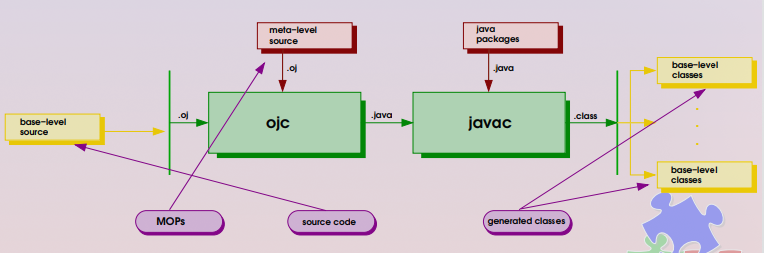
\includegraphics[scale=0.3]{14-openjava}
\end{center}

\subsubsection{How OpenJava Translates the Program: The OpenJava MOP}

\textbf{Before compiling the source,}

\begin{itemize}
	\item the compiler invokes the method translate() of the meta-object at the root of the program AST
\end{itemize}

\begin{center}
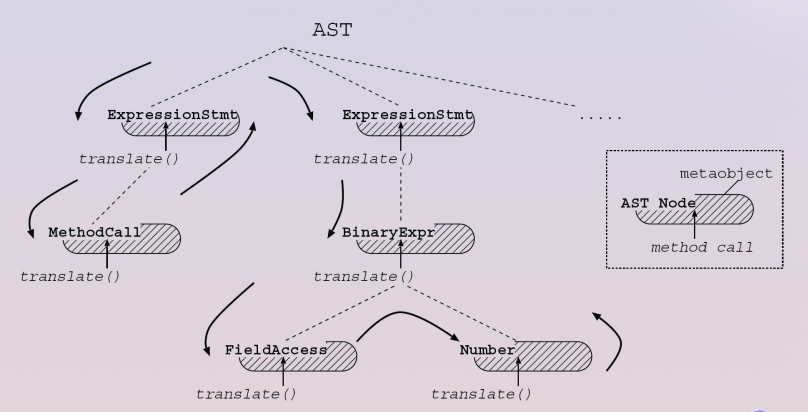
\includegraphics[scale=0.3]{14-openjava-2}
\end{center}

\textbf{The method}

\begin{itemize}
	\item recursively walks the AST translating the code (type-driven visit)
\end{itemize}

\textbf{Language extensions are implemented by redefining the translate() method in the corresponding class}

\subsubsection{Characteristics}

Openjava works on a per-class basis associating to every class another class (the meta-object) that governs the translation process.

Meta-objects and objects interact through a well-defined MOP.

The OpenJava’s work is based on a Java to Java translation

The meta-objects represent the program in execution in the meta-level.

\subsubsection{How to Program with OpenJava}

\textbf{Reflective programming in OpenJava mainly takes three steps:}

\begin{itemize}
	\item we have to decide how the base-level program has to look after the translation; then
	\item we have to detect which part of the base-level code will be involved in the translation and to decide which ancillary code is necessary during the translation; and
	\item we have to write a meta-object that will carry out the designed translation.
\end{itemize}

Notwithstanding that the translation is carried out at compiletime, the reflective API is very simple and looks like the one provided by java.lang.reflect.

\subsubsection{Example: Verbose Execution}

\begin{lstlisting}[language=Java]
public class Hello instantiates VerboseClass {
	public static void main( String[] args ) {
		hello();
	}
	static void hello() {
		System.out.println( "Hello, world." );
	}
}
\end{lstlisting}

The base-level code, excluding the instantiates statement, is pure Java code.

The statement:

\begin{lstlisting}[language=Java]
instantiates VerboseClass
\end{lstlisting}

says to the compiler that the class Hello has a meta-object instance of the class VerboseClass

The class VerboseClass describes how the class Hello has to be translated

\subsubsection{Example: Verbose Execution (Cont'd)}

In the example

\begin{itemize}
	\item we want to print a message at every method call,
	\item so we can imagine that the code, after the translation, should look like this:
\end{itemize}

\begin{lstlisting}[language=Java]
public class Hello {
	public static void main( String[] args ) {
		System.out.println( "main is called." );
		hello();
	}
	static void hello() {
		System.out.println( "hello is called." );
		System.out.println( "Hello, world." );
	}
}
\end{lstlisting}

Figured out how the code should look we have to write a metaobject to do that

\subsubsection{Example: Verbose Execution (Cont'd)}

VerboseClass verbose-izes the execution of the Hello instances

\begin{lstlisting}[language=Java]
import openjava.mop.*;
import openjava.ptree.*;
public class VerboseClass instantiates Metaclass extends OJClass {
	public void translateDefinition() throws MOPException {
		OJMethod[] methods = getDeclaredMethods();
		for (int i = 0; i < methods.length; ++i) {
			Statement printer = makeStatement(
			"System.out.println( " + methods[i] + "\" is called.\" );"
			);
			methods[i].getBody().insertElementAt( printer, 0 );
		}
	}
}
\end{lstlisting}

\begin{lstlisting}[language=Java]
[18:57]cazzola@hymir:~/tsp> java Hello
main is called.
hello is called.
Hello, world.
\end{lstlisting}

\subsubsection{Example: Verbose Execution (Cont'd)}

To enable such a translation, the class VerboseClass:

\begin{itemize}
	\item extends the class openjava.mop.OJClass;
	\item overrides the method translateDefinition() that translates the body of the methods;
	\item the methods declared in the base-level classes are retrieved thanks to a call to the getDeclaredMethods();
	\item the call to the method makeStatement() allows to build a statement from a string on-the-fly;
	\item the method getBody() returns a list of statements representing the body of the method; statements can be added to or removed from that representation.
\end{itemize}



